% !TEX TS-program = knitr
\documentclass[handout]{beamer}\usepackage{graphicx, color}
%% maxwidth is the original width if it is less than linewidth
%% otherwise use linewidth (to make sure the graphics do not exceed the margin)
\makeatletter
\def\maxwidth{ %
  \ifdim\Gin@nat@width>\linewidth
    \linewidth
  \else
    \Gin@nat@width
  \fi
}
\makeatother

\IfFileExists{upquote.sty}{\usepackage{upquote}}{}
\definecolor{fgcolor}{rgb}{0.2, 0.2, 0.2}
\newcommand{\hlnumber}[1]{\textcolor[rgb]{0,0,0}{#1}}%
\newcommand{\hlfunctioncall}[1]{\textcolor[rgb]{0.501960784313725,0,0.329411764705882}{\textbf{#1}}}%
\newcommand{\hlstring}[1]{\textcolor[rgb]{0.6,0.6,1}{#1}}%
\newcommand{\hlkeyword}[1]{\textcolor[rgb]{0,0,0}{\textbf{#1}}}%
\newcommand{\hlargument}[1]{\textcolor[rgb]{0.690196078431373,0.250980392156863,0.0196078431372549}{#1}}%
\newcommand{\hlcomment}[1]{\textcolor[rgb]{0.180392156862745,0.6,0.341176470588235}{#1}}%
\newcommand{\hlroxygencomment}[1]{\textcolor[rgb]{0.43921568627451,0.47843137254902,0.701960784313725}{#1}}%
\newcommand{\hlformalargs}[1]{\textcolor[rgb]{0.690196078431373,0.250980392156863,0.0196078431372549}{#1}}%
\newcommand{\hleqformalargs}[1]{\textcolor[rgb]{0.690196078431373,0.250980392156863,0.0196078431372549}{#1}}%
\newcommand{\hlassignement}[1]{\textcolor[rgb]{0,0,0}{\textbf{#1}}}%
\newcommand{\hlpackage}[1]{\textcolor[rgb]{0.588235294117647,0.709803921568627,0.145098039215686}{#1}}%
\newcommand{\hlslot}[1]{\textit{#1}}%
\newcommand{\hlsymbol}[1]{\textcolor[rgb]{0,0,0}{#1}}%
\newcommand{\hlprompt}[1]{\textcolor[rgb]{0.2,0.2,0.2}{#1}}%

\usepackage{framed}
\makeatletter
\newenvironment{kframe}{%
 \def\at@end@of@kframe{}%
 \ifinner\ifhmode%
  \def\at@end@of@kframe{\end{minipage}}%
  \begin{minipage}{\columnwidth}%
 \fi\fi%
 \def\FrameCommand##1{\hskip\@totalleftmargin \hskip-\fboxsep
 \colorbox{shadecolor}{##1}\hskip-\fboxsep
     % There is no \\@totalrightmargin, so:
     \hskip-\linewidth \hskip-\@totalleftmargin \hskip\columnwidth}%
 \MakeFramed {\advance\hsize-\width
   \@totalleftmargin\z@ \linewidth\hsize
   \@setminipage}}%
 {\par\unskip\endMakeFramed%
 \at@end@of@kframe}
\makeatother

\definecolor{shadecolor}{rgb}{.97, .97, .97}
\definecolor{messagecolor}{rgb}{0, 0, 0}
\definecolor{warningcolor}{rgb}{1, 0, 1}
\definecolor{errorcolor}{rgb}{1, 0, 0}
\newenvironment{knitrout}{}{} % an empty environment to be redefined in TeX

\usepackage{alltt}
\newcommand{\answers}{1}

\usetheme{Marburg}
\setbeamertemplate{navigation symbols}{} 
\setbeamercovered{dynamic}
\setbeamertemplate{footline}
{
  \leavevmode%
  \hbox{%
  \begin{beamercolorbox}[wd=.333333\paperwidth,ht=2.25ex,dp=1ex,center]{author in head/foot}%
    \usebeamerfont{author in head/foot}\copyright $\ $ \insertshortauthor%~~\beamer@ifempty{\insertshortinstitute}{}{(\insertshortinstitute)}
  \end{beamercolorbox}%
  \begin{beamercolorbox}[wd=.333333\paperwidth,ht=2.25ex,dp=1ex,center]{title in head/foot}%
    \usebeamerfont{title in head/foot} \insertinstitute
  \end{beamercolorbox}%
  \begin{beamercolorbox}[wd=.333333\paperwidth,ht=2.25ex,dp=1ex,right]{date in head/foot}%
    \usebeamerfont{date in head/foot}\insertshortdate{}\hspace*{2em}
    \insertframenumber{} / \inserttotalframenumber\hspace*{2ex} 
  \end{beamercolorbox}}%
  \vskip0pt%
}

\usepackage{amsmath}
\usepackage{caption}
\usepackage{color}
\usepackage{enumerate}
\usepackage{listings}
\usepackage{hyperref}
\usepackage{mathrsfs}
\usepackage{natbib}
\usepackage{url}

\providecommand{\all}{\ \forall \ }
\providecommand{\bs}{\backslash}
\providecommand{\e}{\varepsilon}
\providecommand{\E}{\ \exists \ }
\providecommand{\lm}[2]{\lim_{#1 \rightarrow #2}}
\providecommand{\m}[1]{\mathbb{#1}}
\providecommand{\nv}{{}^{-1}}
\providecommand{\ov}[1]{\overline{#1}}
\providecommand{\p}{\newpage}
\providecommand{\q}{$\quad$ \newline}
\providecommand{\rt}{\rightarrow}
\providecommand{\Rt}{\Rightarrow}
\providecommand{\vc}[1]{\boldsymbol{#1}}
\providecommand{\wh}[1]{\widehat{#1}}

\hypersetup{colorlinks,linkcolor=,urlcolor=blue}
\numberwithin{equation}{section}

\definecolor{dkgreen}{rgb}{0,0.6,0}
\definecolor{gray}{rgb}{0.5,0.5,0.5}
\definecolor{mauve}{rgb}{0.58,0,0.82}

\lstset{ 
  language=C,                % the language of the code
  basicstyle= \footnotesize,           % the size of the fonts that are used for the code
  numberstyle= \tiny \color{white},  % the style that is used for the line-numbers
  stepnumber=2,                   % the step between two line-numbers. 
  numbersep=5pt,                  % how far the line-numbers are from the code
  backgroundcolor=\color{white},      % choose the background color. You must add \usepackage{color}
  showspaces=false,               % show spaces adding particular underscores
  showstringspaces=false,         % underline spaces within strings
  showtabs=false,                 % show tabs within strings adding particular underscores
  frame=lrb,                   % adds a frame around the code
  rulecolor=\color{black},        % if not set, the frame-color may be changed on line-breaks within not-black text 
  tabsize=2,                      % sets default tabsize to 2 spaces
  captionpos=t,                   % sets the caption-position 
  breaklines=true,                % sets automatic line breaking
  breakatwhitespace=false,        % sets if automatic breaks should only happen at whitespace
  %title=\lstname,                   % show the filename of files included with \lstinputlisting;
  keywordstyle=\color{blue},          % keyword style
  commentstyle=\color{gray},       % comment style
  stringstyle=\color{dkgreen},         % string literal style
  escapeinside={\%*}{*)},            % if you want to add LaTeX within your code
  morekeywords={*, ...},               % if you want to add more keywords to the set
  xleftmargin=0.053in, % left horizontal offset of caption box
  xrightmargin=-.03in % right horizontal offset of caption box
}

%\DeclareCaptionFont{white}{\color{white}}
%\DeclareCaptionFormat{listing}{\parbox{\textwidth}{\colorbox{gray}{\parbox{\textwidth}{#1#2#3}}\vskip-0.05in}}
%\captionsetup[lstlisting]{format = listing, labelfont = white, textfont = white}
%For caption-free listings, comment out the 3 lines above and uncomment the 2 lines below.
 \captionsetup{labelformat = empty, labelsep = none}
 \lstset{frame = single}




\title{Descriptive Statistics: Part 1/2 (Ch 3)}
\author{Will Landau}
\date{January 24, 2013}
\institute{Iowa State University}

\begin{document}

\begin{frame}
\titlepage
 \end{frame}
 
 \AtBeginSection[]
{
   \begin{frame}
       \frametitle{Outline}
       \tableofcontents[currentsection]
   \end{frame}
}

\section{What is descriptive statistics?}

\begin{frame}
\frametitle{What is descriptive statistics?}

\begin{itemize}
\pause \item {\bf Descriptive statistics}: the use of plots and numerical summaries to describe data without drawing any formal conclusions.
\pause \item Descriptive statistics seeks to find the following features of datasets:
\begin{itemize}
\pause \item Center: the point that the data are closest to on average
\pause \item Spread: how wide the data look, how varied the points are
\pause \item Shape (more on that when we get to plots)
\pause \item Outliers: points that lie way beyond the rest of the data.
\end{itemize}
\end{itemize}

\end{frame}


\section{Graphical and Tabular Displays}

\subsection{Dot diagrams}

\begin{frame}
\frametitle{Gear data}
\begin{center}
\setkeys{Gin}{width=.75\textwidth} 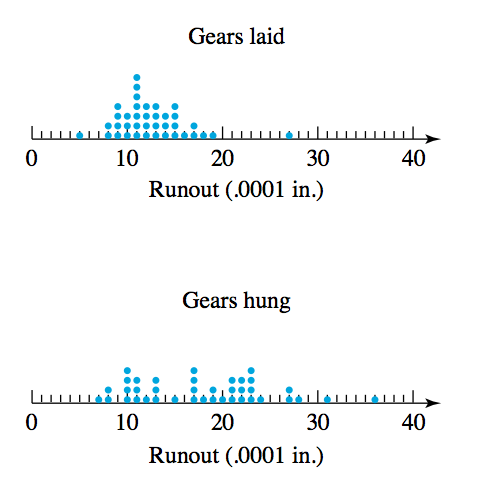
\includegraphics{../../fig/geardot.png}
\end{center}
\end{frame}

\begin{frame}
\frametitle{New example: bullet data}
\begin{center}
\setkeys{Gin}{width=1\textwidth} 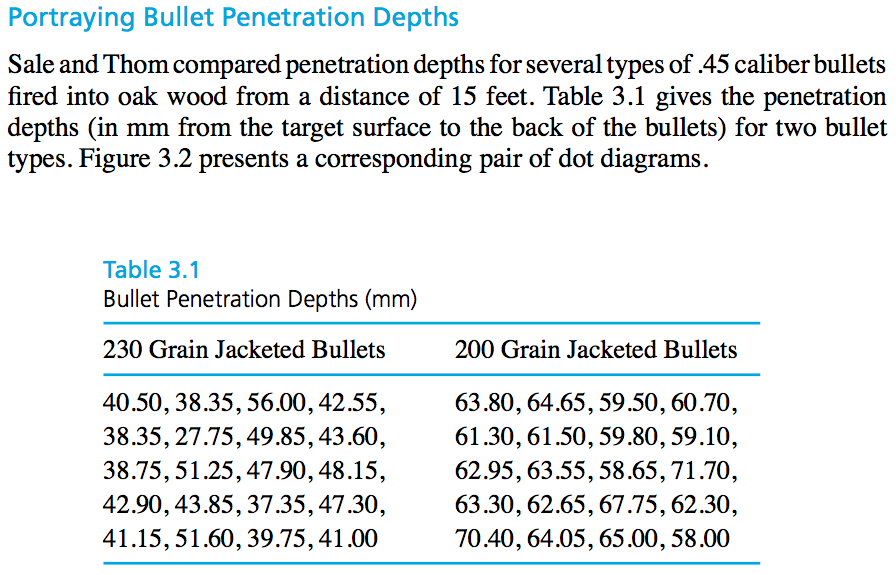
\includegraphics{../../fig/bulletdata.png}
\end{center}
\end{frame}

\begin{frame}
\frametitle{Gear data}
\begin{center}
\setkeys{Gin}{width=.75\textwidth} 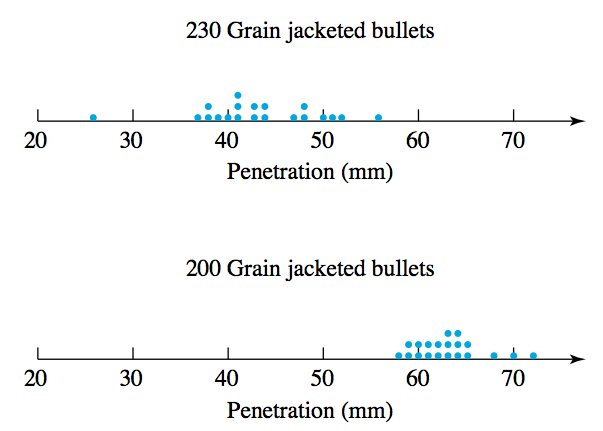
\includegraphics{../../fig/bulletdot.png}
\end{center}
\end{frame}



\subsection{Stem and leaf plots}

\begin{frame}
\frametitle{Stem and leaf plots: laid gears}
\begin{center}
\setkeys{Gin}{width=1\textwidth} 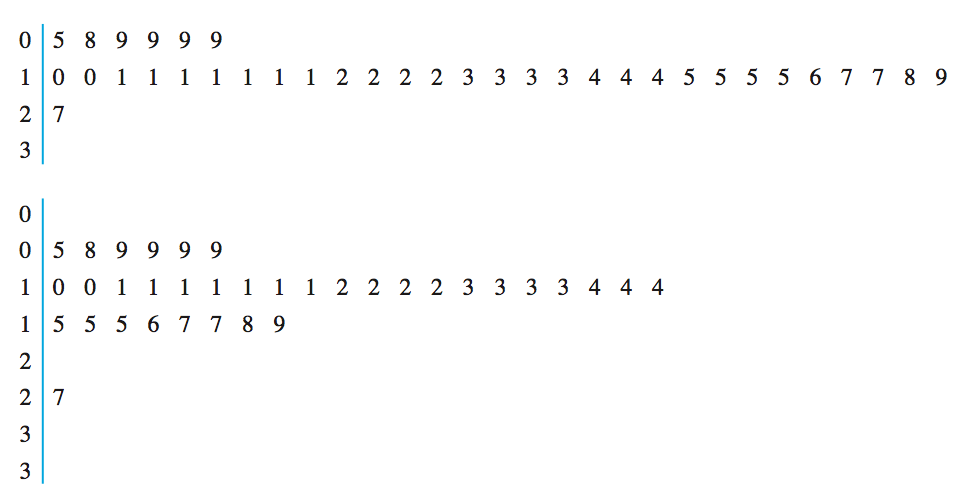
\includegraphics{../../fig/gearstemlaid.png}
\end{center}
\end{frame}


\begin{frame}
\frametitle{Back to back stem and leaf plots}
\begin{center}
\setkeys{Gin}{width=1\textwidth} 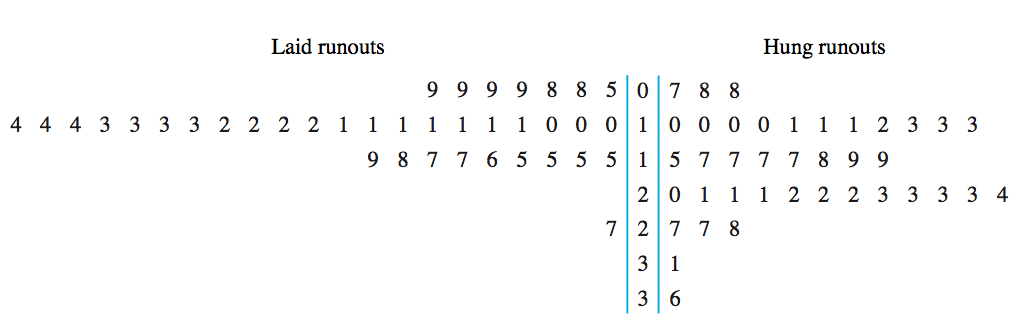
\includegraphics{../../fig/gearstemback2back.png}
\end{center}
\end{frame}

\subsection{Frequency tables}

\begin{frame}
\frametitle{Frequency Table: gear data}
\begin{center}
\setkeys{Gin}{width=1\textwidth} 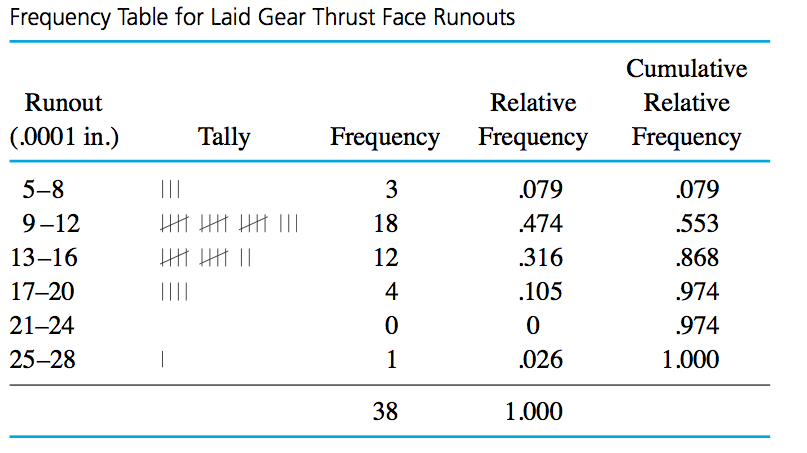
\includegraphics{../../fig/gearfreq.png}
\end{center}
\end{frame}

\begin{frame}
\frametitle{Frequency Table: bullet data, 200 grain}
\begin{center}
\setkeys{Gin}{width=1\textwidth} 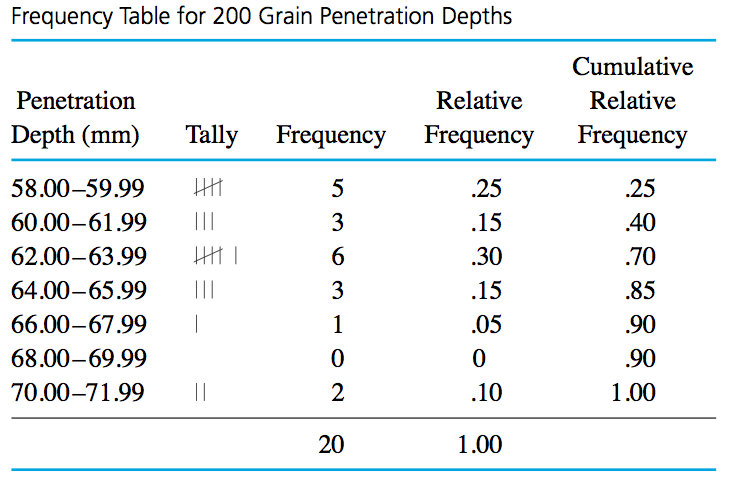
\includegraphics{../../fig/bulletsfreq.png}
\end{center}
\end{frame}

\subsection{Histograms}

\begin{frame}
\frametitle{Histogram: bullet data, 200 grain}
\begin{center}
\setkeys{Gin}{width=.85\textwidth} 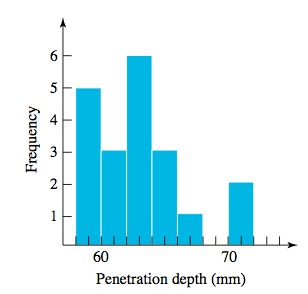
\includegraphics{../../fig/bullethist.png}
\end{center}
\end{frame}

\begin{frame}
\frametitle{Histogram guidelines}
\setkeys{Gin}{width=1\textwidth} 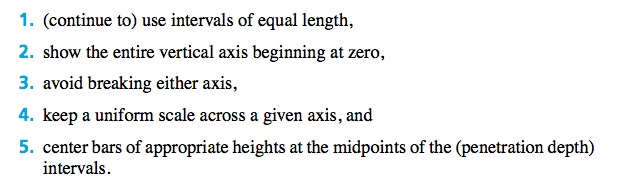
\includegraphics{../../fig/histrules.png}
\begin{itemize}
\pause \item Also: histograms are for continuous data only. The equivalent plot for discrete and categorical data is called a \emph{bar plot}, featured next. 
\end{itemize}
\end{frame}

\subsection{Bar plots}

\begin{frame}[fragile]
\frametitle{Discrete data: cars} \scriptsize
\begin{knitrout}
\definecolor{shadecolor}{rgb}{0.969, 0.969, 0.969}\color{fgcolor}\begin{kframe}
\begin{verbatim}
## % latex table generated in R 2.15.1 by xtable 1.7-0 package
## % Mon Feb 25 23:40:38 2013
## \begin{table}[ht]
## \begin{center}
## \begin{tabular}{rll}
##   \hline
##  & mpg & cyl \\ 
##   \hline
## Mazda RX4 & 21 & 6 \\ 
##   Mazda RX4 Wag & 21 & 6 \\ 
##   Datsun 710 & 22.8 & 4 \\ 
##   Hornet 4 Drive & 21.4 & 6 \\ 
##   Hornet Sportabout & 18.7 & 8 \\ 
##   Valiant & 18.1 & 6 \\ 
##   Duster 360 & 14.3 & 8 \\ 
##   Merc 240D & 24.4 & 4 \\ 
##   Merc 230 & 22.8 & 4 \\ 
##   Merc 280 & 19.2 & 6 \\ 
##   Merc 280C & 17.8 & 6 \\ 
##   Merc 450SE & 16.4 & 8 \\ 
##   Merc 450SL & 17.3 & 8 \\ 
##   Merc 450SLC & 15.2 & 8 \\ 
##   Cadillac Fleetwood & 10.4 & 8 \\ 
##   ... & ... & ... \\ 
##    \hline
## \end{tabular}
## \end{center}
## \end{table}
\end{verbatim}
\end{kframe}
\end{knitrout}

\end{frame}


\begin{frame}
\frametitle{Discrete data frequency table: cars data}

\begin{tabular}{|c|c|c|c|}
\hline
Cylinders & Freq. & Relative Freq. & Cumulative Rel. Freq.\\ \hline
4 & 11 & 0.344 & 0.344 \\ \hline
6 & 7 & 0.219 & 0.563 \\ \hline
8 & 14 & 0.4375 & 1\\ \hline
\end{tabular}
\end{frame}


\begin{frame}[fragile]
\frametitle{Bar plot (not a histogram)}
\begin{knitrout}
\definecolor{shadecolor}{rgb}{0.969, 0.969, 0.969}\color{fgcolor}
\includegraphics[width=\maxwidth]{figure/unnamed-chunk-3} 

\end{knitrout}

\end{frame}



\subsection{Scatterplots}

\begin{frame}[fragile]
\frametitle{Bivariate data: cars}
\begin{knitrout}
\definecolor{shadecolor}{rgb}{0.969, 0.969, 0.969}\color{fgcolor}\begin{kframe}
\begin{verbatim}
## % latex table generated in R 2.15.1 by xtable 1.7-0 package
## % Mon Feb 25 23:40:38 2013
## \begin{table}[ht]
## \begin{center}
## \begin{tabular}{rll}
##   \hline
##  & mpg & wt \\ 
##   \hline
## Mazda RX4 & 21 & 2.62 \\ 
##   Mazda RX4 Wag & 21 & 2.875 \\ 
##   Datsun 710 & 22.8 & 2.32 \\ 
##   Hornet 4 Drive & 21.4 & 3.215 \\ 
##   Hornet Sportabout & 18.7 & 3.44 \\ 
##   Valiant & 18.1 & 3.46 \\ 
##   Duster 360 & 14.3 & 3.57 \\ 
##   Merc 240D & 24.4 & 3.19 \\ 
##   Merc 230 & 22.8 & 3.15 \\ 
##   Merc 280 & 19.2 & 3.44 \\ 
##   Merc 280C & 17.8 & 3.44 \\ 
##   Merc 450SE & 16.4 & 4.07 \\ 
##   Merc 450SL & 17.3 & 3.73 \\ 
##   Merc 450SLC & 15.2 & 3.78 \\ 
##   Cadillac Fleetwood & 10.4 & 5.25 \\ 
##   ... & ... & ... \\ 
##    \hline
## \end{tabular}
## \end{center}
## \end{table}
\end{verbatim}
\end{kframe}
\end{knitrout}

\end{frame}

\begin{frame}[fragile]
\frametitle{Scatterplot: mpg vs wt, cats data}
\begin{knitrout}
\definecolor{shadecolor}{rgb}{0.969, 0.969, 0.969}\color{fgcolor}
\includegraphics[width=\maxwidth]{figure/unnamed-chunk-5} 

\end{knitrout}

\end{frame}

\begin{frame}
\frametitle{Distributional shapes}
Why do we plot data? To see the distributional shape. \q
\setkeys{Gin}{width=1\textwidth} 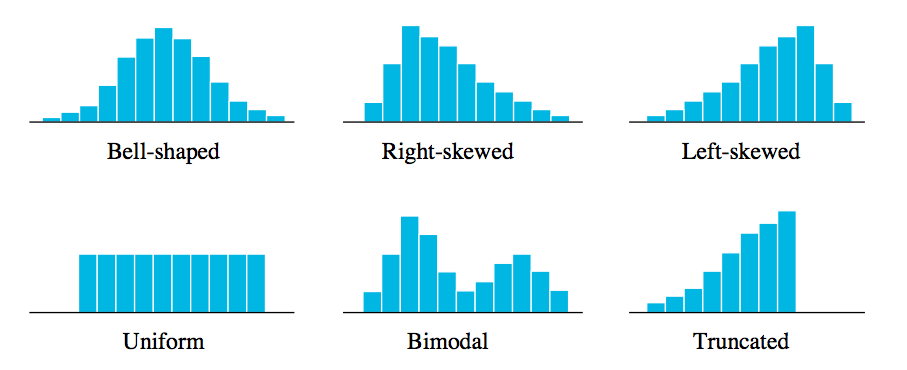
\includegraphics{../../fig/distshapes.png}
\end{frame}

\section{Quantiles}

\begin{frame}
\frametitle{Percentiles and quantiles}
\begin{itemize}
\item {\bf The $p$'th percentile of a dataset}: a number greater than $p$ \% of the data and less than the rest.
\begin{itemize}
\pause \item ``You scored at the 90'th percentile on the SAT" means that your score was higher than 90\% of the students who took the test and lower than the other 10\%
\pause \item ``Zorbit was positioned at the 80th percentile of the list of fastest growing companies compiled by INC magazine." means Zorbit was growing faster than 80\% of the companies in the list and below the other 20\%. 
\end{itemize}
\pause \item {\bf The $p$ quantile of a dataset}: a percentile, except with $p$ expressed as a decimal number, not a percentage.
\begin{itemize}
\pause \item ``You scored at the 0.9 quantile on the SAT" 
\pause \item ``Zorbit was positioned at the 0.8 quantile of the list compiled by INC magazine."
\end{itemize}
\end{itemize}
\end{frame}


\begin{frame}
\frametitle{Calculating quantiles of finite datasets: setup}

\begin{itemize}
\item Given:
\begin{itemize}
\item $x_1, \ldots x_n$, an ordered list of numbers. This is the dataset.
\pause \item $p$, a number between 0 and 1.
\end{itemize}
\pause \item Goal: calculate $Q(p)$, the $p$ quantile of the dataset.
\pause \item Notation:
\begin{itemize}
 \item $Q(p)$ is called the {\bf quantile function}.
\pause \item $\lfloor x \rfloor$ is called the {\bf \href{http://en.wikipedia.org/wiki/Floor\_and\_ceiling\_functions}{floor function}}. 
\pause \item $\lceil x \rceil$ is called the {\bf \href{http://en.wikipedia.org/wiki/Floor\_and\_ceiling\_functions}{ceiling function}}. 
\end{itemize}

\end{itemize}
\end{frame}




\begin{frame}
\frametitle{Calculating quantiles of finite datasets: procedure}
\begin{enumerate}[1. ]
\item Let $p_i = \frac{i-.5}{n}, \ i = 1, \ldots, n$ 
\pause \item Define $Q(p_i) = x_i $ for $i = 1, \ldots n$.
\begin{enumerate}[a. ]
\pause \item If $p = p_j$ for some index $j$, then $Q(p) = Q(p_j)$.
\pause \item Otherwise, linearly interpolate $Q(p)$:
\begin{enumerate}[i. ]
\pause \item Let $i' = np+.5$ (Solve $p = \frac{i'-.5}{n}$ for $i'$).
\pause \item Take $Q(p) = (\lceil i' \rceil -i')x_{\lfloor i' \rfloor} + (i'-\lfloor i' \rfloor)x_{\lceil i' \rceil}$ 
\end{enumerate}
\end{enumerate}
\end{enumerate}
\end{frame}











\begin{frame}[fragile]
\frametitle{Example: breaking strength (g) of towels}

\begin{knitrout}
\definecolor{shadecolor}{rgb}{0.969, 0.969, 0.969}\color{fgcolor}\begin{kframe}
\begin{verbatim}
## % latex table generated in R 2.15.1 by xtable 1.7-0 package
## % Mon Feb 25 23:40:38 2013
## \begin{table}[ht]
## \begin{center}
## \begin{tabular}{cc}
##   \hline
## test & strength \\ 
##   \hline
##   1 & 8577 \\ 
##     2 & 9471 \\ 
##     3 & 9011 \\ 
##     4 & 7583 \\ 
##     5 & 8572 \\ 
##     6 & 10688 \\ 
##     7 & 9614 \\ 
##     8 & 9614 \\ 
##     9 & 8527 \\ 
##    10 & 9165 \\ 
##    \hline
## \end{tabular}
## \end{center}
## \end{table}
\end{verbatim}
\end{kframe}
\end{knitrout}


\end{frame}

\begin{frame}[fragile]
\frametitle{Example: breaking strength (g) of towels}

\begin{knitrout}
\definecolor{shadecolor}{rgb}{0.969, 0.969, 0.969}\color{fgcolor}\begin{kframe}
\begin{verbatim}
## % latex table generated in R 2.15.1 by xtable 1.7-0 package
## % Mon Feb 25 23:40:38 2013
## \begin{table}[ht]
## \begin{center}
## \begin{tabular}{ccc}
##  test & $\frac{i - .5}{10}$ & $i$'th smallest data point, $x_i = Q(\frac{i - .5}{10})$ \\ 
##   \hline
##   1 & 0.05 & 7583 \\ 
##     2 & 0.15 & 8527 \\ 
##     3 & 0.25 & 8572 \\ 
##     4 & 0.35 & 8577 \\ 
##     5 & 0.45 & 9011 \\ 
##     6 & 0.55 & 9165 \\ 
##     7 & 0.65 & 9471 \\ 
##     8 & 0.75 & 9614 \\ 
##     9 & 0.85 & 9614 \\ 
##    10 & 0.95 & 10688 \\ 
##   \end{tabular}
## \end{center}
## \end{table}
\end{verbatim}
\end{kframe}
\end{knitrout}


\end{frame}


\begin{frame}[fragile]
\frametitle{\small Your turn: calculate $Q(0.5), Q(0.18)$, and $Q(0.94)$.} \small

\begin{knitrout}
\definecolor{shadecolor}{rgb}{0.969, 0.969, 0.969}\color{fgcolor}\begin{kframe}
\begin{verbatim}
## % latex table generated in R 2.15.1 by xtable 1.7-0 package
## % Mon Feb 25 23:40:38 2013
## \begin{table}[ht]
## \begin{center}
## \begin{tabular}{ccc}
##  test & $\frac{i - .5}{10}$ & $i$'th smallest data point, $x_i = Q(\frac{i - .5}{10})$ \\ 
##   \hline
##   1 & 0.05 & 7583 \\ 
##     2 & 0.15 & 8527 \\ 
##     3 & 0.25 & 8572 \\ 
##     4 & 0.35 & 8577 \\ 
##     5 & 0.45 & 9011 \\ 
##     6 & 0.55 & 9165 \\ 
##     7 & 0.65 & 9471 \\ 
##     8 & 0.75 & 9614 \\ 
##     9 & 0.85 & 9614 \\ 
##    10 & 0.95 & 10688 \\ 
##   \end{tabular}
## \end{center}
## \end{table}
\end{verbatim}
\end{kframe}
\end{knitrout}


\begin{enumerate}[$\text{Case}$ 1.  ]
\item Define $Q(p_i) = x_i $ for $i = 1, \ldots n$.
\item If $p \ne p_i$ for any $i$, linearly interpolate $Q(p)$:
\begin{enumerate}[a. ]
\item Let $i' = np+.5$ (Solve $p = \frac{i'-.5}{n}$ for $i'$)
\item Take $Q(p) = (\lceil i' \rceil -i')x_{\lfloor i' \rfloor} + (i'-\lfloor i' \rfloor)x_{\lceil i' \rceil}$ 
\end{enumerate}
\end{enumerate} 
\end{frame}

\begin{frame}<handout:\answers>
\frametitle{Q(0.5)}
\begin{align*}
i' &= np + .5 \\
& \uncover<2->{=10 \cdot 0.5 + 0.5 = 5.5}\\ \\
\uncover<3->{Q(0.5)} &   \uncover<3->{=(\lceil i' \rceil -i')x_{\lfloor i' \rfloor} + (i'-\lfloor i' \rfloor)x_{\lceil i' \rceil}} \\
&\uncover<4->{= (\lceil 5.5 \rceil - 5.5)x_{\lfloor 5.5 \rfloor} + (5.5 - \lfloor 5.5 \rfloor)x_{\lceil 5.5 \rceil}} \\
&\uncover<5->{= (6 - 5.5) x_5 + (5.5 - 5) x_6} \\
&\uncover<6->{= (0.5) 9011 + (0.5) 9165} \\
&\uncover<7->{= 9088}
\end{align*}
\end{frame}

\begin{frame}<handout:\answers>
\frametitle{Q(0.18)}
\begin{align*}
i' &= np + .5 \\
&\uncover<2->{=10 \cdot 0.18 + 0.5 = 2.3} \\ \\
\uncover<3->{Q(0.18)} &\uncover<3->{=   (\lceil i' \rceil -i')x_{\lfloor i' \rfloor} + (i'-\lfloor i' \rfloor)x_{\lceil i' \rceil} }\\
&\uncover<4->{=(\lceil 2.3 \rceil - 2.3)x_{\lfloor 2.3 \rfloor} + (2.3 - \lfloor 2.3 \rfloor)x_{\lceil 2.3 \rceil}} \\
& \uncover<5->{= (3 - 2.3) x_2 + (2.3 - 2) x_3} \\
& \uncover<6->{= (0.7) 8527 + (0.3) 8572} \\
&\uncover<7->{= 8540.5}
\end{align*}
\end{frame}

\begin{frame}<handout:\answers>
\frametitle{Q(0.94)}
\begin{align*}
i' &= np + .5 \\
&\uncover<2->{=10 \cdot 0.94 + 0.5 = 9.9 }\\ \\
\uncover<3->{Q(0.94)} &\uncover<3->{=   (\lceil i' \rceil -i')x_{\lfloor i' \rfloor} + (i'-\lfloor i' \rfloor)x_{\lceil i' \rceil}} \\
&\uncover<4->{=(\lceil 9.9 \rceil - 9.9)x_{\lfloor 9.9 \rfloor} + (9.9 - \lfloor 9.9 \rfloor)x_{\lceil 9.9 \rceil}} \\
&\uncover<5->{ = (10 - 9.9) x_9 + (9.9 - 9) x_{10}} \\
&\uncover<6->{ = (0.1) 9614+ (0.9)10688 } \\
&\uncover<7->{= 10580.6}
\end{align*}
\end{frame}


\begin{frame}
\frametitle{More on quantiles}

\begin{itemize}
\item Special quantiles:
\begin{itemize}
\item {\bf Minimum}: $Q\left ( \frac{1 - .5}{n}\right)$
\pause \item {\bf Lower Quartile}: $Q(0.25)$
\pause \item {\bf Median}: $Q(0.5)$
\pause \item {\bf Upper Quartile}: $Q(0.75)$
\pause \item {\bf Maximum}: $Q\left ( \frac{n - .5}{n} \right ) $
\end{itemize}
\pause \item {\bf Interquartile Range (IQR)}: $Q(0.75) - Q(0.25)$
\begin{itemize}
\pause \item Most points should be below $Q(0.75) + 1.5 \cdot $IQR and above $Q(0.25) - 1.5 \cdot$ IQR. 
\item {\bf Outlier}: a point above $Q(0.75) + 1.5 \cdot $IQR or below $Q(0.25) - 1.5 \cdot$ IQR. 
\end{itemize}
\end{itemize}
\end{frame}

%\begin{frame}
%\frametitle{Sources}
%\begin{enumerate}[1. ]
%\item Some source
%\end{enumerate}
%\end{frame}

\end{document}
